\documentclass{beamer}
\usepackage[utf8]{inputenc}
\usepackage[T1]{fontenc}
\usepackage[italian]{babel}

\usetheme{Boadilla}		% see http://deic.uab.es/~iblanes/beamer_gallery/
\usecolortheme{default}	% see http://deic.uab.es/~iblanes/beamer_gallery/
%\useoutertheme[]{smoothbars}
\useinnertheme{circles}
%\usefonttheme{structuresmallcapsserif}
\setbeamercovered{dynamic}
	% boxes - seahorse, Boadilla - seahorse, CambridgeUS - default
%\setbeamercolor{background canvas}{bg=white}	& posso selezionare i colori per ogni elemento
%\setbeamertemplate{background canvas}[vertical shading][bottom=white,top=structure.fg!10]	% ci sono altri template

%\usepackage{pgfpages}
%\pgfpagesuselayout{4 on 1}[a4paper,border shrink=5mm,landscape]
\setbeamertemplate{footline}[frame number]{}
\setbeamertemplate{navigation symbols}{}

\usepackage{amsfonts}
\usepackage{mathtools,physics}

\theoremstyle{definition}
\newtheorem{definizione}{Definizione}
\theoremstyle{plain}
\newtheorem{teorema}{Teorema}

\usepackage{xcolor}  %colori

\usepackage{verbatim}
\usepackage{lipsum}

\usepackage{booktabs}
\usepackage{subfig}
\usepackage{float}

\usepackage[italian, sort, noabbrev, capitalise]{cleveref}
\usepackage[bottom]{footmisc}

\usepackage[cdot, thickqspace, squaren]{SIunits}

% macro
\def\code#1{\texttt{#1}}

\title{Termalizzazione in sistemi quantistici}
\subtitle{il principio canonico generale}
\author[Alessandro Candido]{\texorpdfstring{Alessandro Candido\\Relatore: dr. Davide Rossini}{Alessandro Candido}}
\institute{}
%\logo{\includegraphics[width=15mm]{sigillo}}
%\titlegraphic{\includegraphics{hfigurai}

\date{\today}

\begin{document}

\begin{frame}
	\maketitle
\end{frame}

\begin{frame}
	\transpush[direction = 180]<1>
	\frametitle{Indice}
	\tableofcontents
\end{frame}

\section{Stato termico}
\begin{frame}
	\transpush[direction = 180]<1>
	\transwipe<2->
	\frametitle{Requisiti per uno stato termico}
	
	Per un sistema in uno stato termico:
	\begin{itemize}[<+->]
		\item i valori delle osservabili del sistema devono essere stazionari;
		\item lo stato asintotico non deve dipendere strettamente dalle condizioni iniziali.
	\end{itemize}
\end{frame}

\section{Ipotesi ergodica}
\begin{frame}
	\transpush[direction = 180]<1>
	\frametitle{L'ipotesi ergodica}
	\centering
	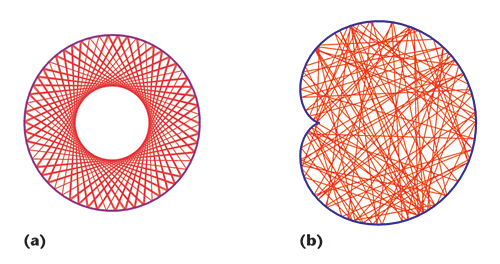
\includegraphics[width=0.8\columnwidth]{./Images/ErgodicHypothesis.png}
	
	Un sistema non ergodico (a) ed uno ergodico (b).
\end{frame}

\begin{frame}
	\transpush[direction = 180]<1>
	\transwipe<2->
	\frametitle{L'ipotesi ergodica}
	
	\begin{block}{Meccanica classica}
		L'ipotesi ergodica è ben definita: essa afferma che il sistema esplora ogni regione accessibile dello spazio delle fasi per un tempo proporzionale alla sua area.
	\end{block}
	\pause
	\begin{alertblock}{Meccanica quantistica}
		 \textbf{Il sistema non perde memoria.}
		 
		 Infatti, nella base degli stati stazionari l'evoluzione temporale:
		 \begin{itemize}[<+->]
		 	\item fa oscillare le fasi, con frequenze fissate dalle rispettive energie;
		 	\item ma \textbf{conserva le ampiezze} (i moduli).
		 \end{itemize}
	\end{alertblock}

	% \'E importante che>
	% - in meccanica classica le equazioni del moto sono del secondo ordine, per questo motivo l'evoluzione temporale fa sì che i sistemi siano quasi sempre (tranne insiemi a misura nulla, senza fonte) ergodici, cioè se non lo sono è sufficiente una piccola perturbazione (interazione) per renderli tali
	% - in meccanica quantistica l'evoluzione temporale è lineare, questo porta ad un gran numero di quantità conservate quasi sempre (tranne un insieme a misura nulla), cioè tutte le ampiezze sugli stati stazionari, e le differenze di fase fra stati degeneri: è questo fatto a creare il problema della termalizzazione
\end{frame}

\begin{frame}
	\transpush[direction = 180]<1>
	\transwipe<2->
	\frametitle{L'ipotesi ergodica}
	
	Per spiegare il fatto che anche i sistemi quantistici termalizzino è stato proposto di spostare l'attenzione \textbf{dagli stati alle osservabili} \hyperlink{bib}{(von Neumann, 1929)}.
	
	\pause
	\begin{block}{\hyperlink{termdef2}{Termalizzazione}}
		Fissato un insieme \textbf{minimale} di osservabili macroscopiche, $\{ M_\beta \}$ si richiede che:
		\begin{equation*}
			\overline{\bra{\Psi(t)} M_\beta \ket{\Psi(t)}} = \Tr[M_\beta \hat{\rho}_{diag}] = \expval{M_\beta}_{mc}
		\end{equation*}
		{\footnotesize La media nel tempo è effettuata per tempi lunghi rispetto alle energie coinvolte (cioè i periodi di oscillazione delle fasi).}
	\end{block}
	
	\pause
	Il problema si sposta quindi sulla definizione di un insieme \textbf{minimale} di osservabili macroscopiche, cioè il \textit{macrostato} del sistema.
\end{frame}

\section{Comportamento asintotico}
\begin{frame}
	\transpush[direction = 180]<1>
	\transwipe<2->
	\frametitle{Ergodicità e termalizzazione}
	\framesubtitle{In sistemi quantistici}
	\hypertarget{overview}{}
	
	\`E stato dimostrato, teoricamente e sperimentalmente, che alcuni sistemi quantistici isolati \textbf{non termalizzano}.
	
	\pause
	L'avvenire della termalizzazione per tempi lunghi sembra essere collegato all'\textbf{integrabilità} del sistema.
	
	\pause
	Sono stati studiati allora più modi per descrivere e spiegare lo stato asintotico, termico e non, dei sistemi quantistici:
	
	\pause
	\begin{itemize}[<+->]
		\item \hyperlink{GGE}{ensemble di Gibbs generalizzati};
		\item \hyperlink{ETH}{\textit{Eigenstate Thermalzation Hypothesis}};
		\item \textbf{principio canonico generale} \hyperlink{bib}{(Popescu, 2006)}.
	\end{itemize}

	Si prenderà in esame quest'ultimo argomento.

	% Il senso di questa slide è esporre un punto di vista d'insieme:
	% - il problema della statistica quantistica è stato esposto nelle slide precedenti
	% - i GGE sono un modo per convivere con il problema: accetti che siano conservate altre quantità oltre all'energia
	% - ETH è un modo per spiegare perché la termalizzazione avvenga anche in meccanica quantistica, perché se alla fine il mondo è quantistico la termalizzazione ci deve essere (la si osserva)
	% - il principio canonico generale: è un modo per evitare in toto il problema dell'equiprobabilità a priori e dell'ipotesi ergodica
\end{frame}

\section{Il principio canonico generale}

\begin{frame}[allowframebreaks]
	\transpush[direction = 180]
	\frametitle{Definizioni}
	
	\begin{block}{Sistema}
		Il sistema in esame è un sottosistema, S, di un sistema quantistico isolato, detto \textit{universo}, sottoposto a un insieme di vincoli, R.
		
		La porzione residua dell'universo è detta ambiente, E.
	\end{block}
	
	Si avranno allora:
	\begin{itemize}
		\item $\mathcal{H}_R$, lo spazio di Hilbert dell'universo con dimensione $d_R$;
		\item $\mathcal{H}_E$, lo spazio di Hilbert dell'ambiente con dimensione $d_E$;
		\item $\mathcal{H}_S$, lo spazio di Hilbert del sottosistema con dimensione $d_S$.
	\end{itemize}
	
	E sarà:
	\begin{equation*}
	\mathcal{H}_R \subseteq \mathcal{H}_S \otimes \mathcal{H}_E
	\end{equation*}
	
	\pagebreak
	
	Lo stato di un sottosistema è ottenuto tracciando lo stato del sistema sui gradi di libertà complementari al sottosistema.
	\begin{block}{Stato canonico}
		Si definisce lo stato canonico del sottosistema, $\Omega_S$:
		\begin{equation*}
		\Omega_S = \Tr_E \mathcal{E}_R
		\end{equation*}
		Dove $\mathcal{E}$ è lo stato misto \textit{equiprobabile} dell'universo:
		\begin{equation*}
		\mathcal{E}_R = \frac{1}{d_R} \mathbf{1}_R
		\end{equation*}
	\end{block}
	
	Lo stato del sistema corrispondente allo stato $\ket{\varphi}$ dell'universo sarà:
	\begin{equation*}
	\rho_S = \Tr_E \ket{\varphi}\bra{\varphi}
	\end{equation*}
\end{frame}


\begin{frame}
	\transpush[direction = 180]<1>
	\frametitle{Il principio canonico generale}
	
	\begin{block}{Enunciato}
		Dato un sottosistema sufficientemente piccolo di un sistema quantistico isolato, detto \textit{universo}, per quasi ogni stato puro dell'universo il sottosistema è approssimativamente nello stato canonico $\Omega_S$.
		\newline
		
		Cioè, per quasi ogni $\ket{\varphi} \in \mathcal{H}_R$:
		\begin{equation*}
			\rho_S \approx \Omega_S
		\end{equation*}
		
	\end{block}

	Il \textit{principio canonico generale} si propone di \textbf{rimpiazzare} l'ipotesi di \textit{equiprobabilità a priori}, e conseguentemente anche la stessa \textit{ipotesi ergodica}, nel caso di sottosistemi.
\end{frame}

\begin{frame}
	\transpush[direction = 180]<1>
	\transwipe<2->
	\frametitle{Remarks}
	
	Va notato che il principio canonico generale: %forse è meglio trovare dell'altro italiano
	\begin{itemize}
		\item \textbf{non pone limiti al tipo di vincoli} da imporre (l'energia stessa può non essere conservata, il sistema può essere altamente integrabili, \dots);
		\item \textbf{non indaga la natura di $\Omega_S$}, che non è vincolato a essere in una forma alla Boltzmann.
	\end{itemize}

	\pause
	\begin{exampleblock}{Esempi}
		\begin{itemize}
			\item per interazioni deboli fra \textbf{S} e \textbf{E} si recupera il caso canonico imponendo come vincolo \textbf{R} la sola conservazione dell'energia $\mathfrak{E}$.
			\begin{equation*}
				\Omega_S(\mathfrak{E}) \propto \exp\left( - \frac{H_S}{k_B T(\mathfrak{E})}\right)
			\end{equation*}
			\pause
			\item non imponendo alcun vincolo si ottiene:
			\begin{equation*}
			\Omega_S(\mathfrak{E}) \propto \mathbf{1}_R
			\end{equation*}
			che può essere interpretato come un ensemble canonico con $T \rightarrow \infty$
		\end{itemize}
	\end{exampleblock}
\end{frame}

\begin{frame}
	\transpush[direction = 180]<1>
	\transwipe<2->
	\frametitle{Il principio canonico generale}
	\framesubtitle{Teorema}
	\hypertarget{th}{}
	
	Il principio canonico generale è un teorema:
	
	\pause
	\begin{description}[<+->]
		\item[Ipotesi] L'unica ipotesi è che il sottosistema sia sufficientemente piccolo.
		\item[Tesi] La tesi è \hyperlink{LevyLemma}{\textbf{quantitativa}}:
		\begin{block}{}
			\begin{equation*}
				\frac{V[\{\ket{\varphi} \in \mathcal{H}_R | D(\rho_S(\ket{\varphi}), \Omega_S) \geq \eta\}]}{V[\{\ket{\varphi} \in \mathcal{H}_R\}]} \leq \eta'
			\end{equation*}
			con:
			\begin{equation*}
			\eta = \epsilon + \frac{1}{2} \sqrt{\frac{d_S}{d_E^{eff}}} \qquad	\eta' = 4\exp(-Cd_R\epsilon^2)	\qquad	\qquad	\epsilon > 0
			\end{equation*}
		\end{block}
		\pause[4]
	Poiché per ipotesi $d_S \ll d_E^{eff}$ si ottiene $\eta, \eta' \ll 1$ scegliendo, ad esempio, $\epsilon = d_R^{-1/3}$ (poiché $d_s \geq 1$ allora $d_R \gg 1$).
	\end{description}
\end{frame}

\begin{frame}
	\transpush[direction = 180]<1>
	\transwipe<2->
	\frametitle{Il principio canonico generale}
	\framesubtitle{Spiegazione delle quantità usate}
	
	\begin{itemize}[<+->]
		\item L'espressione $V[\cdot]$ è il volume (la misura) dell'insieme all'interno dello spazio di Hilbert $\mathcal{H}_R$.
		\item L'espressione $D(\cdot,\cdot)$ è la distanza della traccia:
		\begin{equation*}
			D(\rho_S, \Omega_S) = \frac{1}{2} \Tr \sqrt{(\rho_S - \Omega_S)^\dagger(\rho_S - \Omega_S)}
		\end{equation*}
		
		usata in questo contesto per quantificare la distanza tra i due stati, essa infatti è la massima differenza nella probabilità di ottenere una certa misura (un certo valore per una data osservabile).
		\item $C$ è una costante, e vale $(2/9)\pi^{-3}$
		\item $d_E^{eff}$ è la dimensione efficace dell'ambiente (\textit{slide successiva}).
	\end{itemize}
\end{frame}

\begin{frame}
	\transpush[direction = 180]<1>
	\frametitle{Il principio canonico generale}
	\framesubtitle{Spiegazione delle quantità usate}
	
	\centering
	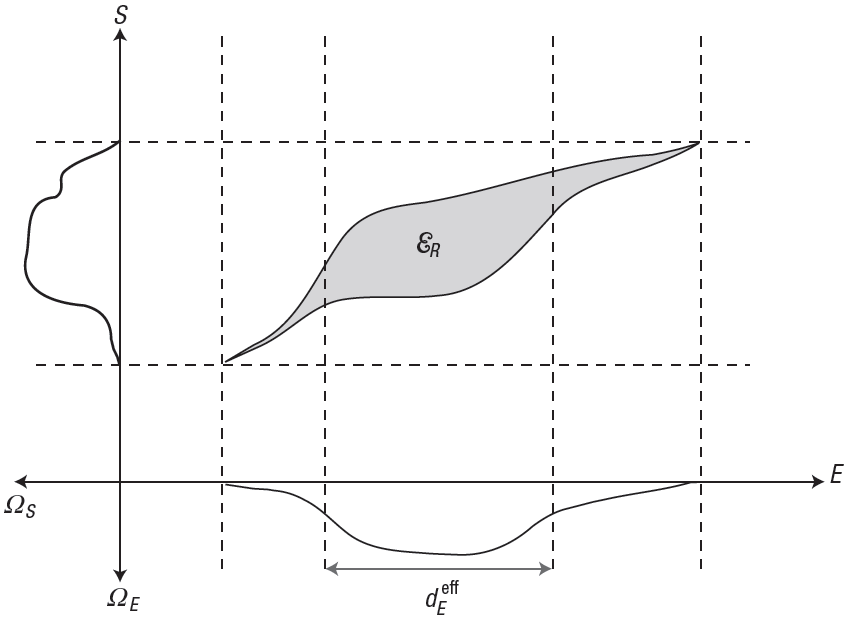
\includegraphics[width=0.8\textwidth]{./Images/popescu(deff).png}
\end{frame}

\section{Bibliografia}
\begin{frame}[allowframebreaks]
	\transpush[direction = 180]
	\frametitle{\refname}
	\hypertarget{bib}{}
		
	\begin{thebibliography}{9}
		\bibitem[von Neumann, 1929]{vonneumann1929} 
		von Neumann, John
		\newblock \emph{Beweis des Ergodensatzes und des H-Theorems in der neuen Mechanik}
		\newblock {Zeitschrift fuer Physik, Vol. 57, 1929, p. 30-70}
		
		\bibitem[Polkovnikov, 2011]{polkovnikov2011}
		Polkovnikov, Anatoli; Sengupta, Krishnendu; Silva, Alessandro; Vengalattore, Mukund
		\newblock \emph{Colloquium: Nonequilibrium dynamics of closed interacting quantum systems}
		\newblock {Review of Modern Phyics, Vol. 83, No. 3, 08.2011, p. 863-883}
		
		\bibitem[Popescu, 2006]{popescu2006} 
		Popescu, Sandu; Short, Anthony J.; Winter, Andreas
		\newblock \emph{Entanglement and the foundations of statistical mechanics}
		\newblock {Nature Physics, Vol. 2, No. 11, 11.2006, p. 754-758}
		
		\bibitem[Reimann, 2006]{reimann2006} 
		Reimann, Peter
		\newblock \emph{Foundation of Statistical Mechanics under Experimentally Realistic Conditions}
		\newblock {Physical Review Letters, Vol. 101, No. 19, 11.2008, 190403}
		
		\bibitem[Reimann, 2006]{reimann2006} 
		Milman, Vitali D.; Schechtman, Gideon
		\newblock \emph{Asymptotic Theory of Finite-Dimensional Normed Spaces}
		\newblock {Ch. 2, 5–6 and 140–141 Appendix V, Lecture Notes in Mathematics, Vol. 1,200, Springer, Berlin, 1986}
	\end{thebibliography}
\end{frame}

\begin{frame}
	\transwipe
	\frametitle{L'ipotesi ergodica}
	\hypertarget{termdef2}{}
	
	
	La definizione di \textit{termalizzazione} che si è data non è del tutto naturale, perché si deve specificare bene la scala temporale su cui si fanno le medie: 
	\begin{itemize}
		\item grande rispetto ai tempi tipici degli stati stazionari;
		\item piccola o comparabile rispetto ai tempi di osservazione.
	\end{itemize}
	
	Una definizione forse più naturale sarebbe stata:
	\begin{block}{Termalizzazione, definizione alternativa}
		Fissato un insieme \textbf{minimale} di osservabili macroscopiche, $\{ M_\beta \}$ si richiede che:
		\begin{equation*}
		\expval{M_\beta}_{\Psi(t)} \longrightarrow_{t \rightarrow + \infty} \expval{M_\beta}_{mc}
		\end{equation*}
	\end{block}

	Il motivo per cui non è stata scelta questa è che ci sarebbero problemi con il \textit{revival} quantistico \hyperlink{bib}{(Reimann, 2008)}.
	
	Si può superare il problema imponendo che la media della distanza si annulli, ma si reintroduce il concetto di media.
\end{frame}

\begin{frame}
	\transwipe
	\frametitle{Ensemble di Gibbs generalizzati}
	\hypertarget{GGE}{}
	
	\hyperlink{overview}{}
	\alert{citare Jaynes e forse qualcun altro (vedere Polkovnikov)}
\end{frame}

\begin{frame}
	\transwipe
	\frametitle{Eigenstate Thermalization Hypothesis}
	\hypertarget{ETH}{}
	
	\hyperlink{overview}{}
	\alert{Citare Srednicky, è lui che l'ha messa su}
\end{frame}

\begin{frame}
	\transwipe
	\frametitle{Il lemma di Levy}
	\hypertarget{LevyLemma}{}
	
	\begin{columns}
		\begin{column}{0.6\textwidth}
			Il \hyperlink{th}{teorema} esposto si fonda su un risultato matematico nell'ambito della geometria in dimensione alta, noto come Lemma di Levy (Milman, 1986).
			
			\alert{Piccola spiegazione del contenuto del lemma (va bene quella in didascalia nell'articolo di Popescu)}
		\end{column}
		\begin{column}{0.4\textwidth}
			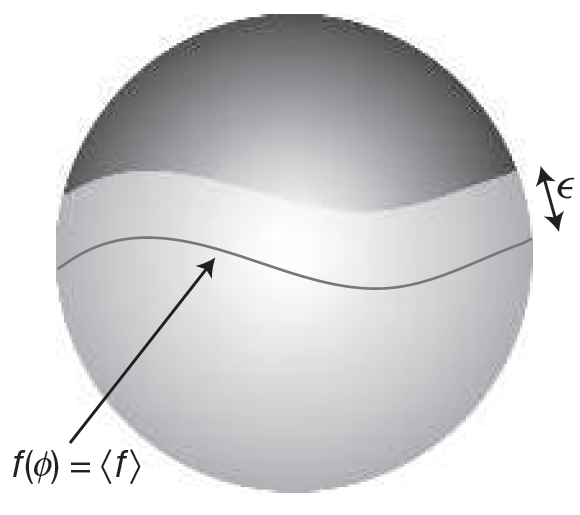
\includegraphics[width=\columnwidth]{./Images/Levy2D.png}
			
			{\footnotesize Illustrazione del caso 2D del lemma di Levy, in cui è evidente che il risultato sia molto diverso da quello richiesto a causa della bassa dimensionalità.}
		\end{column}
	\end{columns}
	
	\alert{Leggere articolo di conti di Popescu}
\end{frame}

\end{document}